%==============================================================================
%  RoadVision — Sprawozdanie z projektu zespołowego
%  Przedmiot: Projekt Zespołowy
%  Uczelnia: Wyższa Szkoła Informatyki i Zarządzania w Rzeszowie (WSIiZ)
%
%  UWAGA: Strona tytułowa poniżej jest TYMCZASOWYM PLACEHOLDEREM.
%         Należy ją zastąpić oficjalnym wzorem strony tytułowej WSIiZ.
%==============================================================================
\documentclass[14pt,a4paper]{extarticle}

\usepackage[T1]{fontenc}
\usepackage[utf8]{inputenc}
\usepackage[polish]{babel}
\usepackage{newtxtext}   % Times New Roman (tekst)
\usepackage{newtxmath}   % Times New Roman (matematyka)
\usepackage[a4paper,margin=2.4cm]{geometry}

\usepackage{graphicx}
\usepackage[table]{xcolor}
\usepackage{booktabs}
\usepackage{array}
\usepackage{tabularx}
\usepackage{longtable}
\usepackage{multirow}
\usepackage{enumitem}
\usepackage{float}
\usepackage{caption}
\usepackage{listings}
\usepackage{titlesec}
\usepackage{fancyhdr}
\usepackage{indentfirst}

% Klasyczny wcięcie akapitowe (interlinia domyślna)
\setlength{\parindent}{1.25cm}
\setlength{\parskip}{0pt}
\setlength{\emergencystretch}{3em}  % ogranicza wystawanie wierszy poza margines

\usepackage{tikz}
\usetikzlibrary{shapes.geometric, arrows.meta, positioning, calc, fit,
                backgrounds, shadows.blur, decorations.pathreplacing, trees}
\usepackage{pgfgantt}
\usepackage{pgf-pie}

\usepackage[hidelinks]{hyperref}

% Polskie babel uaktywnia znak ", a my używamy „cudzysłowów” bezpośrednio.
\shorthandoff{"}

%-------------------------- Kolory marki RoadVision ---------------------------
\definecolor{rvBlue}{HTML}{1F4E79}
\definecolor{rvCyan}{HTML}{2E86AB}
\definecolor{rvGreen}{HTML}{2E8B57}
\definecolor{rvOrange}{HTML}{E07B39}
\definecolor{rvRed}{HTML}{C0392B}
\definecolor{rvGray}{HTML}{5D6D7E}
\definecolor{rvLight}{HTML}{EAF2F8}
\definecolor{rvLightGreen}{HTML}{E8F6EF}
\definecolor{rvLightOrange}{HTML}{FCF3E8}
\definecolor{rvHead}{HTML}{D9DDE1}   % formalna szarość — nagłówki tabel, elementy grupujące

%-------------------------------- Nagłówki (czarne) ---------------------------
\titleformat{\section}{\color{black}\Large\bfseries}{\thesection.}{0.6em}{}
\titleformat{\subsection}{\color{black}\large\bfseries}{\thesubsection.}{0.5em}{}
\titleformat{\subsubsection}{\color{black}\normalsize\bfseries}{\thesubsubsection.}{0.5em}{}

\pagestyle{fancy}
\fancyhf{}
\fancyhead[L]{\small\color{rvGray}Projekt Zespołowy}
\fancyhead[R]{\small\color{rvGray}WSIiZ}
\fancyfoot[C]{\thepage}
\renewcommand{\headrulewidth}{0.4pt}

% Podpisy: wyśrodkowane, kursywa; etykieta pogrubiona, czarna
\captionsetup{font={small,it}, labelfont={bf}, labelsep=period,
              justification=centering, singlelinecheck=true}

%-------------------------------- Listingi ------------------------------------
\definecolor{codebg}{HTML}{F7F9FB}
\definecolor{codekw}{HTML}{1F4E79}
\definecolor{codestr}{HTML}{2E8B57}
\definecolor{codecom}{HTML}{8C95A0}
\lstdefinestyle{py}{
  language=Python,
  backgroundcolor=\color{codebg},
  basicstyle=\ttfamily\scriptsize,
  keywordstyle=\color{codekw}\bfseries,
  stringstyle=\color{codestr},
  commentstyle=\color{codecom}\itshape,
  numbers=left, numberstyle=\tiny\color{rvGray}, numbersep=8pt,
  frame=single, rulecolor=\color{rvLight},
  breaklines=true, showstringspaces=false,
  tabsize=2, columns=fullflexible,
  literate={ą}{{\k a}}1 {ć}{{\'c}}1 {ę}{{\k e}}1 {ł}{{\l}}1 {ń}{{\'n}}1
           {ó}{{\'o}}1 {ś}{{\'s}}1 {ż}{{\.z}}1 {ź}{{\'z}}1
}

% Skróty do bloczków TikZ
\tikzset{
  rvnode/.style={rectangle, rounded corners=3pt, draw=rvBlue, line width=0.8pt,
                 fill=rvLight, text=rvBlue, font=\small\bfseries, align=center,
                 minimum width=2.4cm, minimum height=1cm, blur shadow={shadow blur steps=4}},
  rvflow/.style={-{Stealth[length=2.5mm]}, line width=1pt, color=rvGray},
}

\newcommand{\rvchip}[2]{\tikz[baseline=-0.6ex]\node[fill=#1,text=white,rounded corners=2pt,
   inner sep=2pt,font=\scriptsize\bfseries]{#2};}

% Placeholder na zrzut ekranu.
%  Użycie:  \zrzut{nazwa_pliku.png}{wysokość}{opis czego dotyczy zrzut}
%  Aby wstawić prawdziwy obraz, zastąp wywołanie poleceniem:
%      \includegraphics[width=0.8\textwidth]{img/nazwa_pliku.png}
\newcommand{\zrzut}[3]{%
  \setlength{\fboxsep}{0pt}%
  \fcolorbox{rvGray}{rvHead!35}{%
    \begin{minipage}[c][#2][c]{0.8\textwidth}\centering
      {\color{rvGray}\itshape [\,Miejsce na zrzut ekranu\,]}\\[6pt]
      {\color{black}\small #3}\\[6pt]
      {\color{rvGray}\ttfamily\footnotesize \detokenize{img/#1}}
    \end{minipage}}}

%==============================================================================
\begin{document}

%--------------------------- STRONA TYTUŁOWA (wzór WSIiZ) ---------------------
\begin{titlepage}
\centering
\vspace*{0.6cm}

\includegraphics[width=0.46\textwidth]{img/wsiiz_logo.png}\\[2.4cm]

{\Large Sprawozdanie z realizacji projektu}\\[2.2cm]

{\LARGE\bfseries System monitorowania\\[0.2cm]
jakości nawierzchni drogowej\\[0.2cm]
w czasie rzeczywistym}\\[2.4cm]

{\Large\scshape Projekt Zespołowy}\\[3.0cm]

\vfill
\noindent\begin{minipage}[t]{0.5\textwidth}
\raggedright
\textbf{Prowadzący:}\\[0.15cm]
mgr inż. Aleksander Mysakowec
\end{minipage}%
\begin{minipage}[t]{0.5\textwidth}
\raggedleft
\textbf{Wykonawcy:}\\[0.15cm]
Roman Bezshchasnyi, Grupa P1, 69930\\
Rostysław Yaremko, Grupa P1, 69958
\end{minipage}\\[1.6cm]

{\large Rzeszów 2026}
\end{titlepage}

%--------------------------------- SPIS TREŚCI --------------------------------
\tableofcontents
\thispagestyle{fancy}
\newpage

%==============================================================================
\section{Wprowadzenie}
%==============================================================================

\subsection{Cel i geneza projektu}
Stan nawierzchni dróg miejskich bezpośrednio wpływa na bezpieczeństwo uczestników
ruchu, komfort jazdy oraz koszty eksploatacji pojazdów. Tradycyjna inwentaryzacja
ubytków (dziur, wybojów, miejsc gwałtownego hamowania) prowadzona jest ręcznie,
jest kosztowna i szybko traci aktualność. Celem projektu RoadVision było
zaprojektowanie i zbudowanie działającego systemu, który automatycznie gromadzi
dane z czujników pojazdu, w czasie rzeczywistym klasyfikuje stan nawierzchni i
prezentuje wynik na interaktywnej mapie miasta.

System przygotowaliśmy jako rozwiązanie pilotażowe dla obszaru Rzeszowa, z
możliwością łatwej rekonfiguracji na dowolny inny obszar — współrzędne mapy oraz
źródło danych są zwykłymi parametrami konfiguracyjnymi.

\subsection{Cel dokumentu}
Sprawozdanie pełni dwie role. Po pierwsze, opisuje sposób, w jaki zorganizowaliśmy
pracę dwuosobowego zespołu — przyjętą metodykę, podział prac (WBS), harmonogram,
analizę ścieżki krytycznej, zarządzanie ryzykiem oraz kontrolę postępów. Po drugie,
przedstawia rozwiązanie techniczne — architekturę, model danych, algorytmy oraz
gotowy produkt. Zgodnie z charakterem przedmiotu Projekt Zespołowy najwięcej uwagi
poświęciliśmy pierwszemu obszarowi.

\subsection{Zakres i założenia}
\begin{itemize}[leftmargin=1.4em, itemsep=2pt]
  \item Akwizycja danych z czterech źródeł: akcelerometr, GPS, czujnik
        temperatury/wilgotności oraz dane o zajętości parkingów.
  \item Klasyfikacja stanu nawierzchni do jednej z kategorii: \rvchip{rvGreen}{równa},
        \rvchip{rvOrange}{wyboj}, \rvchip{rvRed}{dziura}, \rvchip{rvGray}{gwałtowne hamowanie}.
  \item Przetwarzanie strumieniowe w architekturze brzegowej (edge computing).
  \item Trwałe składowanie danych oraz dystrybucja w czasie rzeczywistym
        (WebSocket) do aplikacji wizualizującej.
  \item Pełna konteneryzacja środowiska uruchomieniowego (Docker Compose).
\end{itemize}

%==============================================================================
\section{Zespół projektowy i organizacja pracy}
%==============================================================================

\subsection{Skład zespołu i podział obowiązków}
Projekt realizowaliśmy we dwóch. Na początku podzieliliśmy się obowiązkami tak,
aby każdy zajął się tym, co lubi i robi sprawniej, ale zostawiliśmy też kilka
obszarów wspólnych — dzięki temu żaden moduł nie był znany tylko jednej osobie.
Z grubsza podział wyglądał tak: Roman wziął na siebie część serwerową i
infrastrukturę, a Rostysław stronę kliencką i prezentację danych. Staraliśmy się,
żeby ilość pracy rozłożyła się po połowie.

\begin{table}[H]
\centering
\caption{Podział obowiązków w zespole}
\renewcommand{\arraystretch}{1.3}
\begin{tabularx}{\textwidth}{>{\bfseries}p{3.2cm} X}
\toprule
\rowcolor{rvHead}\textbf{Osoba} & \textbf{Czym się zajmował} \\
\midrule
Roman Bezshchasnyi &
  Architektura systemu, moduł Agent, klasyfikacja nawierzchni (Edge),
  buforowanie danych (Hub, Redis), konteneryzacja (Docker), prowadzenie
  repozytorium i harmonogramu. \\
Rostysław Yaremko &
  Moduł Store (API, baza danych, WebSocket), aplikacja MapView (mapa, trasa,
  markery), klasyfikacja pogody, testy scenariuszowe oraz dokumentacja wraz z
  materiałem graficznym. \\
\bottomrule
\end{tabularx}
\end{table}

\noindent Analizę wymagań i ogólny kształt architektury obmyśliliśmy razem —
to były decyzje, które wpływały na pracę obu osób, więc nie chcieliśmy ich
podejmować w pojedynkę. Część zadań przesuwaliśmy też między sobą w trakcie
semestru, gdy ktoś miał akurat więcej czasu (więcej o tym w sekcji~\ref{sec:zasoby}).

\subsection{Macierz odpowiedzialności RACI}
Żeby nie było wątpliwości, kto za co odpowiada, rozpisaliśmy zadania w prostej
tabeli RACI (Responsible, Accountable, Consulted, Informed).

\begin{table}[H]
\centering
\caption{Macierz RACI dla kluczowych pakietów prac}
\renewcommand{\arraystretch}{1.25}
\begin{tabularx}{\textwidth}{X c c}
\toprule
\rowcolor{rvHead}\textbf{Pakiet pracy} & \textbf{Roman} & \textbf{Rostysław} \\
\midrule
Analiza wymagań i koncepcja systemu        & A/R & C \\
Architektura i interfejsy modułów          & A/R & C \\
Moduł Agent (akwizycja, MQTT)              & A/R & I \\
Moduł Edge (klasyfikacja nawierzchni)      & A/R & I \\
Moduł Hub (Redis, buforowanie)             & A/R & I \\
Moduł Store (API, PostgreSQL, WebSocket)   & C   & A/R \\
Aplikacja MapView (Kivy)                   & I   & A/R \\
Klasyfikacja warunków pogodowych           & I   & A/R \\
Konteneryzacja (Docker Compose)            & A/R & I \\
Testy i scenariusze użycia                 & C   & A/R \\
Dokumentacja i materiał graficzny          & C   & A/R \\
\bottomrule
\end{tabularx}
\end{table}
\noindent\footnotesize R~--~Wykonawca,\quad A~--~Odpowiedzialny (rozliczany),\quad
C~--~Konsultowany,\quad I~--~Informowany.\normalsize

\subsection{Narzędzia współpracy}
\begin{table}[H]
\centering
\caption{Narzędzia wykorzystane do organizacji pracy zespołowej}
\renewcommand{\arraystretch}{1.2}
\begin{tabularx}{\textwidth}{>{\bfseries}p{3.6cm} X}
\toprule
\rowcolor{rvHead}\textbf{Obszar} & \textbf{Narzędzie / metoda} \\
\midrule
Kontrola wersji        & Git + GitHub (gałęzie funkcyjne, Pull Requesty, code review) \\
Zarządzanie zadaniami  & Tablica Kanban (backlog $\rightarrow$ w toku $\rightarrow$ przegląd $\rightarrow$ gotowe) \\
Komunikacja bieżąca    & Komunikator zespołowy + krótkie synchronizacje (stand-up) \\
Środowisko uruchomieniowe & Docker Compose (powtarzalne środowisko dla obu osób) \\
Dokumentacja           & \LaTeX{} (system kontroli wersji wspólny z kodem) \\
\bottomrule
\end{tabularx}
\end{table}

%==============================================================================
\section{Zarządzanie projektem}
%==============================================================================

\subsection{Karta projektu}
Zanim zabraliśmy się do kodu, spisaliśmy na jednej stronie najważniejsze ustalenia:
po co robimy projekt, co dokładnie ma powstać, ile mamy czasu i kiedy uznamy, że
się udało. Ta krótka notatka pomagała nam później wracać do tego, co naprawdę było
ważne.

\begin{table}[H]
\centering
\caption{Karta projektu RoadVision}
\renewcommand{\arraystretch}{1.25}
\begin{tabularx}{\textwidth}{>{\bfseries}p{3.6cm} X}
\toprule
\rowcolor{rvHead}\textbf{Element} & \textbf{Opis} \\
\midrule
Cel             & Zbudowanie działającego systemu monitorowania jakości nawierzchni z wizualizacją w czasie rzeczywistym. \\
Sponsor         & Prowadzący przedmiot Projekt Zespołowy (WSIiZ). \\
Zespół          & 2 osoby (kierownik/architekt, programista/wizualizacja). \\
Czas            & 05.05.2026 -- 09.06.2026 (5 tygodni). \\
Ograniczenia    & Środowisko studenckie, brak realnego sprzętu IoT (dane odtwarzane z CSV). \\
Kryteria sukcesu& Kompletny potok end-to-end, wizualizacja na mapie w czasie rzeczywistym, terminowe oddanie. \\
Poza zakresem   & Produkcyjne wdrożenie, integracja z rzeczywistą flotą pojazdów. \\
\bottomrule
\end{tabularx}
\end{table}

\subsection{Przyjęta metodyka}
Na pierwszym spotkaniu zastanawialiśmy się, czy rozpisać cały projekt „z góry”, czy
raczej pracować małymi krokami. Wyszło nam coś pośredniego. Rzeczy, które trudno
później zmienić — analizę wymagań i ogólną architekturę — przemyśleliśmy dokładnie
na samym początku. Resztę, czyli pisanie kolejnych modułów, podzieliliśmy na
tygodniowe kawałki: pod koniec każdego tygodnia mieliśmy działający fragment i
wspólnie go przeglądaliśmy. Dzięki temu nie musieliśmy nic dużego przerabiać, a
problemy z łączeniem modułów wychodziły szybko.

\begin{figure}[H]
\centering
\resizebox{\textwidth}{!}{%
\begin{tikzpicture}[node distance=0.55cm and 1.0cm]
  \node[rvnode, fill=rvLight] (a){Analiza\\wymagań};
  \node[rvnode, right=of a, fill=rvLight] (b){Projekt\\architektury};
  \node[rvnode, right=of b, fill=rvLightGreen, draw=rvGreen, text=rvGreen] (c){Iteracja 1\\Back-end};
  \node[rvnode, right=of c, fill=rvLightGreen, draw=rvGreen, text=rvGreen] (d){Iteracja 2\\Integracja};
  \node[rvnode, right=of d, fill=rvLightGreen, draw=rvGreen, text=rvGreen] (e){Iteracja 3\\MapView};
  \node[rvnode, right=of e, fill=rvLightOrange, draw=rvOrange, text=rvOrange] (f){Testy +\\dokumentacja};
  \draw[rvflow](a)--(b);\draw[rvflow](b)--(c);\draw[rvflow](c)--(d);
  \draw[rvflow](d)--(e);\draw[rvflow](e)--(f);
  % zwrotne sprzężenie — łuk poprowadzony wyraźnie pod blokami, z dala od ramek
  \draw[rvflow, dashed] (f.south) to[out=-90, in=-90, looseness=0.5] (c.south);
  \node[font=\scriptsize\itshape, text=rvGray]
    at ($(c.south)!0.5!(f.south) + (0,-1.25cm)$) {przegląd / sprzężenie zwrotne};
\end{tikzpicture}}
\caption{Hybrydowy przepływ faz projektu — sekwencyjne planowanie i iteracyjna implementacja.}
\end{figure}

\subsection{Struktura podziału prac (WBS)}
Aby nie zgubić się w zakresie, rozpisaliśmy cały projekt na kartce, a następnie
przenieśliśmy go do formy struktury podziału prac (WBS). Podzieliliśmy całość na
cztery główne pakiety prac, a każdy z nich na drobniejsze zadania — dzięki temu
łatwiej było nam oszacować pracochłonność i zbudować harmonogram. Struktura ta
stała się dla nas punktem wyjścia przy podziale obowiązków między siebie.

\begin{figure}[H]
\centering
\resizebox{\textwidth}{!}{%
\begin{tikzpicture}[
  every node/.style={rounded corners=2pt, draw, align=center, font=\scriptsize,
                     inner sep=3pt, minimum height=6mm},
  level 1/.style={sibling distance=60mm, level distance=14mm},
  level 2/.style={sibling distance=15mm, level distance=16mm},
  edge from parent/.style={draw=rvGray, -{Stealth[length=1.5mm]}}]
  \node[fill=rvGray, text=white, font=\scriptsize\bfseries] {RoadVision}
    child {node[fill=rvLight]{1. Zarządzanie}
      child {node{1.1 Plan}}
      child {node{1.2 Ryzyko}}
      child {node{1.3 Kontrola}}}
    child {node[fill=rvLightGreen]{2. Back-end}
      child {node{2.1 Agent}}
      child {node{2.2 Edge}}
      child {node{2.3 Hub}}
      child {node{2.4 Store}}}
    child {node[fill=rvLightOrange]{3. Front-end}
      child {node{3.1 Mapa}}
      child {node{3.2 Pogoda}}
      child {node{3.3 Trasa}}}
    child {node[fill=rvLight]{4. Wdrożenie}
      child {node{4.1 Docker}}
      child {node{4.2 Testy}}
      child {node{4.3 Dok.}}};
\end{tikzpicture}}
\caption{Struktura podziału prac (Work Breakdown Structure) projektu RoadVision.}
\label{fig:wbs}
\end{figure}

\subsection{Estymacja pracochłonności (metoda trójpunktowa PERT)}
Pracochłonność pakietów oszacowano metodą trójpunktową PERT, w której wartość
oczekiwaną wyznacza się ze wzoru $t_{e}=\frac{o+4m+p}{6}$, gdzie $o$ — szacunek
optymistyczny, $m$ — najbardziej prawdopodobny, $p$ — pesymistyczny (w dniach
roboczych). Podejście to uwzględnia niepewność i ogranicza ryzyko niedoszacowania
(zabezpieczenie R5).

\begin{table}[H]
\centering
\caption{Estymacja pracochłonności metodą PERT (w dniach roboczych)}
\renewcommand{\arraystretch}{1.2}
\begin{tabularx}{\textwidth}{X c c c c}
\toprule
\rowcolor{rvHead}\textbf{Pakiet pracy} & \textbf{$o$} & \textbf{$m$} & \textbf{$p$} & \textbf{$t_e$} \\
\midrule
Analiza wymagań i architektura & 4 & 6 & 9 & 6,2 \\
Moduł Agent                    & 2 & 3 & 5 & 3,2 \\
Moduł Edge (klasyfikacja)      & 3 & 4 & 7 & 4,3 \\
Hub + Store                    & 3 & 5 & 8 & 5,2 \\
Aplikacja MapView              & 5 & 7 & 11 & 7,3 \\
Konteneryzacja i testy         & 3 & 4 & 6 & 4,2 \\
Dokumentacja                   & 3 & 5 & 8 & 5,2 \\
\midrule
\rowcolor{rvHead}\textbf{Razem} & \textbf{23} & \textbf{34} & \textbf{54} & \textbf{35,6} \\
\bottomrule
\end{tabularx}
\end{table}

\subsection{Harmonogram — wykres Gantta}
Realizację zaplanowano na okres od 5 maja do 9 czerwca 2026
(pięć tygodni roboczych). Harmonogram przedstawiono na wykresie Gantta
(rys.~\ref{fig:gantt}); kamienie milowe oznaczono rombami.

\begin{figure}[H]
\centering
\resizebox{\textwidth}{!}{%
\begin{ganttchart}[
  hgrid, vgrid,
  bar height=0.6,
  bar/.append style={fill=rvCyan, draw=rvBlue},
  bar label font=\small,
  group/.append style={fill=rvGray, draw=rvGray},
  group label font=\small\bfseries,
  milestone/.append style={fill=rvOrange, draw=rvRed},
  milestone label font=\small\itshape,
  title/.style={draw=none, fill=rvHead},
  title label font=\small\bfseries,
  link/.style={-{Stealth[length=1.4mm]}, rvGray}
]{1}{36}
  \gantttitle{05--11.05}{7}
  \gantttitle{12--18.05}{7}
  \gantttitle{19--25.05}{7}
  \gantttitle{26.05--01.06}{7}
  \gantttitle{02--09.06}{8} \\
  \ganttgroup{1. Zarządzanie}{1}{36} \\
  \ganttbar{Analiza wymagań}{1}{5} \\
  \ganttmilestone{Zatwierdzenie zakresu}{5} \\
  \ganttbar{Projekt architektury}{5}{9} \\
  \ganttgroup{2. Back-end}{9}{24} \\
  \ganttbar{Agent (MQTT, akwizycja)}{9}{13} \\
  \ganttbar{Edge (klasyfikacja)}{12}{17} \\
  \ganttbar{Hub + Store (Redis, DB)}{16}{21} \\
  \ganttbar{Integracja back-end}{21}{24} \\
  \ganttmilestone{Działający potok danych}{24} \\
  \ganttgroup{3. Front-end}{20}{31} \\
  \ganttbar{MapView (mapa, trasa)}{20}{26} \\
  \ganttbar{Markery + pogoda}{26}{31} \\
  \ganttgroup{4. Wdrożenie}{27}{36} \\
  \ganttbar{Docker Compose}{27}{29} \\
  \ganttbar{Testy scenariuszowe}{30}{34} \\
  \ganttbar{Dokumentacja}{28}{36} \\
  \ganttmilestone{Oddanie projektu}{36}
  \ganttlink{elem2}{elem4}
  \ganttlink{elem9}{elem10}
\end{ganttchart}}
\caption{Harmonogram projektu RoadVision (05.05--09.06.2026) w formie wykresu Gantta.}
\label{fig:gantt}
\end{figure}

\subsection{Kamienie milowe}
\begin{table}[H]
\centering
\caption{Kamienie milowe projektu}
\renewcommand{\arraystretch}{1.2}
\begin{tabularx}{\textwidth}{c >{\bfseries}p{5.2cm} X}
\toprule
\rowcolor{rvHead}\textbf{Data} & \textbf{Kamień milowy} & \textbf{Kryterium akceptacji} \\
\midrule
09.05.2026 & Zatwierdzenie zakresu       & Uzgodniona lista wymagań i kategorii stanu drogi. \\
13.05.2026 & Zamrożenie architektury     & Zdefiniowane interfejsy między modułami. \\
28.05.2026 & Działający potok danych     & Dane przechodzą Agent$\rightarrow$Store bez błędów. \\
04.06.2026 & Kompletny produkt (MVP)     & Wizualizacja na mapie działa w czasie rzeczywistym. \\
09.06.2026 & Oddanie projektu            & Repozytorium i sprawozdanie gotowe do prezentacji. \\
\bottomrule
\end{tabularx}
\end{table}

\subsection{Analiza ścieżki krytycznej (CPM)}
W celu identyfikacji zadań decydujących o terminie zakończenia przeprowadzono
analizę metodą ścieżki krytycznej (CPM). Diagram sieciowy
(rys.~\ref{fig:cpm}) przedstawia zależności między czynnościami; ścieżkę krytyczną
zaznaczono kolorem czerwonym. Każde opóźnienie zadania leżącego na tej ścieżce
przekłada się bezpośrednio na opóźnienie całego projektu (zapas czasu = 0).

\begin{figure}[H]
\centering
\begin{tikzpicture}[
  node distance=1.5cm and 1.4cm,
  act/.style={circle, draw=rvGray, fill=rvLight, minimum size=1.05cm, font=\scriptsize\bfseries, align=center},
  crit/.style={circle, draw=rvRed, line width=1.2pt, fill=rvLightOrange, text=rvRed, minimum size=1.05cm, font=\scriptsize\bfseries, align=center},
  e/.style={-{Stealth[length=2mm]}, rvGray},
  ce/.style={-{Stealth[length=2mm]}, rvRed, line width=1.1pt}]
  \node[crit](A){A\\4d};
  \node[crit, right=of A](B){B\\4d};
  \node[crit, right=of B](C){C\\5d};
  \node[act, above right=0.6cm and 1.3cm of C](D){D\\5d};
  \node[crit, below right=0.6cm and 1.3cm of C](E){E\\5d};
  \node[crit, right=2.6cm of C, yshift=-0.0cm](F){F\\4d};
  \node[crit, right=of F](G){G\\4d};
  \node[crit, right=of G](H){H\\4d};
  \draw[ce](A)--(B); \draw[ce](B)--(C);
  \draw[e](C)--(D); \draw[ce](C)--(E);
  \draw[e](D)-- (F); \draw[ce](E)--(F);
  \draw[ce](F)--(G); \draw[ce](G)--(H);
\end{tikzpicture}
\caption{Diagram sieciowy CPM. Ścieżka krytyczna A--B--C--E--F--G--H (30 dni roboczych) wyróżniona kolorem czerwonym; czynność D (projekt MapView) posiada zapas czasu.}
\label{fig:cpm}
\end{figure}

\noindent\footnotesize
A~--~Analiza wymagań, B~--~Architektura, C~--~Edge (klasyfikacja),
D~--~MapView, E~--~Hub/Store, F~--~Integracja, G~--~Konteneryzacja, H~--~Testy.
\normalsize

\subsection{Zarządzanie zasobami i obciążeniem}
\label{sec:zasoby}
Głównym ograniczonym zasobem w projekcie studenckim jest czas. Aby utrzymać
równomierne obciążenie obu członków zespołu, pracochłonność estymowano dla każdego
pakietu pracy, a następnie bilansowano przydziały. Rozkład szacowanego nakładu
pracy przedstawia rys.~\ref{fig:effort}.

\begin{figure}[H]
\centering
\begin{tikzpicture}
\pie[radius=2.3, text=legend, color={rvBlue, rvGreen, rvOrange, rvGray},
     font=\small, sum=auto]{
  18/Zarządzanie i analiza,
  40/Back-end (Agent--Store),
  27/Front-end (MapView),
  15/Wdrożenie i testy}
\end{tikzpicture}
\caption{Szacunkowy rozkład nakładu pracy według pakietów WBS (\%).}
\label{fig:effort}
\end{figure}

\noindent Staraliśmy się też nie obciążać obu osób naraz: zadania o niższym
priorytecie przesuwaliśmy w obrębie ich zapasu czasu (por.~CPM), żeby uniknąć
tygodni, w których oba moduły wymagałyby intensywnej pracy w tym samym czasie.
Podział obowiązków (opisany w sekcji~2.1) ustaliliśmy tak, aby każdy zajmował się
zadaniami bliższymi jego umiejętnościom — dzięki temu praca szła szybciej.

\subsection{Zarządzanie ryzykiem i techniki zabezpieczające}
Na początku wspólnie wypisaliśmy wszystko, co — naszym zdaniem — mogło pójść nie
tak, a następnie uporządkowaliśmy te zagrożenia w prostym rejestrze ryzyka. Każde
z nich oceniliśmy pod kątem prawdopodobieństwa (P) i wpływu (W) w skali 1--5;
iloczyn $P\!\times\!W$ wyznaczał priorytet reakcji. Dla ryzyk o najwyższym
priorytecie z góry ustaliliśmy, co zrobimy — m.in. redundancję kompetencji,
wczesną integrację oraz powtarzalne środowisko kontenerowe — tak, aby w razie
problemu nie działać w pośpiechu.

\begin{table}[H]
\centering
\caption{Rejestr ryzyka projektu (wybrane pozycje)}
\renewcommand{\arraystretch}{1.25}
\footnotesize
\begin{tabularx}{\textwidth}{p{0.4cm} X c c c X}
\toprule
\rowcolor{rvHead}\textbf{\#} & \textbf{Ryzyko} & \textbf{P} & \textbf{W} & \textbf{P$\times$W} & \textbf{Reakcja / zabezpieczenie} \\
\midrule
R1 & Niedostępność jednego z członków zespołu & 3 & 4 & 12 &
  Redundancja wiedzy (overlap ról), code review, dokumentacja na bieżąco. \\
R2 & Problemy z integracją modułów (MQTT/HTTP/WS) & 4 & 4 & 16 &
  Wczesna integracja „end-to-end”, wspólne kontrakty danych (Pydantic). \\
R3 & Rozbieżność środowisk uruchomieniowych & 3 & 3 & 9 &
  Konteneryzacja Docker Compose — identyczne środowisko dla obu osób. \\
R4 & Błędna kalibracja progów klasyfikacji & 3 & 3 & 9 &
  Parametryzacja progów, testy na danych odtwarzanych z plików CSV. \\
R5 & Niedoszacowanie czasu na dokumentację & 4 & 3 & 12 &
  Rozpoczęcie dokumentacji równolegle z implementacją (od~21.05). \\
R6 & Utrata danych / brak kontroli wersji & 2 & 5 & 10 &
  Repozytorium Git, częste commity, gałęzie funkcyjne. \\
\bottomrule
\end{tabularx}
\normalsize
\end{table}

\begin{figure}[H]
\centering
\begin{tikzpicture}[scale=0.9]
  % tło — każda komórka kolorowana wg iloczynu P×W
  % (zielony: P×W<6, pomarańczowy: 6--12, czerwony: >12)
  \foreach \P in {1,...,5}{
    \foreach \W in {1,...,5}{
      \pgfmathtruncatemacro{\prd}{\P*\W}
      \edef\cc{\ifnum\prd<6 rvGreen\else\ifnum\prd<13 rvOrange\else rvRed\fi\fi}
      \fill[\cc!16] (\P-1,\W-1) rectangle (\P,\W);
    }
  }
  % siatka
  \foreach \x in {0,...,5}{\draw[rvLight](\x,0)--(\x,5);}
  \foreach \y in {0,...,5}{\draw[rvLight](0,\y)--(5,\y);}
  % osie i skala
  \draw[->, rvGray, line width=0.8pt] (0,0)--(5.7,0) node[right,font=\scriptsize]{Prawdop. (P)};
  \draw[->, rvGray, line width=0.8pt] (0,0)--(0,5.7) node[above,font=\scriptsize]{Wpływ (W)};
  \foreach \x in {1,...,5}{\node[font=\tiny,text=rvGray,below] at (\x-0.5,-0.05){\x};}
  \foreach \y in {1,...,5}{\node[font=\tiny,text=rvGray,left]  at (-0.05,\y-0.5){\y};}
  % punkty ryzyka — w środkach komórek, kolor zgodny ze strefą
  \node[fill=rvRed,circle,inner sep=1.6pt,label={[font=\tiny]above:R2}] at (3.5,3.5){};
  \node[fill=rvOrange,circle,inner sep=1.6pt,label={[font=\tiny]above:R1}] at (2.5,3.5){};
  \node[fill=rvOrange,circle,inner sep=1.6pt,label={[font=\tiny]above:R5}] at (3.5,2.5){};
  \node[fill=rvOrange,circle,inner sep=1.6pt,label={[font=\tiny]left:R6}]  at (1.5,4.5){};
  \node[fill=rvOrange,circle,inner sep=1.6pt,label={[font=\tiny]above:R3}] at (2.33,2.5){};
  \node[fill=rvOrange,circle,inner sep=1.6pt,label={[font=\tiny]above:R4}] at (2.67,2.5){};
\end{tikzpicture}
\caption{Macierz ryzyka — pozycjonowanie zagrożeń względem prawdopodobieństwa i wpływu
  (kolor strefy odpowiada iloczynowi P$\times$W). W strefie krytycznej znalazło się
  wyłącznie ryzyko R2.}
\end{figure}

\noindent Rozkład zagrożeń odzwierciedla specyfikę dwuosobowego zespołu: większość
ryzyk ma podwyższony wpływ, ponieważ każdy moduł i każda osoba są dla projektu
kluczowe (brak rezerwy kadrowej). Mimo to tylko jedno ryzyko — trudności z
integracją modułów (R2) — trafiło do strefy krytycznej; pozostałe, dzięki
zaplanowanym z góry zabezpieczeniom, utrzymały się w strefie umiarkowanej.

\subsection{Komunikacja i kontrola postępów}
Komunikację w zespole oparto na krótkich, regularnych synchronizacjach oraz
asynchronicznej wymianie informacji przez komunikator i komentarze w Pull
Requestach. Postęp kontrolowano w cyklu tygodniowym, porównując stan faktyczny z
planem (kamienie milowe). Pomagał w tym wzajemny przegląd kodu — żadna zmiana nie
trafiała do gałęzi głównej bez akceptacji drugiej osoby, co przy okazji realizowało
zabezpieczenie R1 (obie osoby orientowały się w całości projektu).

Postęp śledziliśmy też prostym wykresem wypalania (burndown), porównującym
pozostałą pracę z planem. Rysunek~\ref{fig:burndown} pokazuje, że tempo prac było
zbliżone do planu, z niewielkim przyspieszeniem w ostatnim tygodniu.

\begin{figure}[H]
\centering
\begin{tikzpicture}[scale=1.0]
  % osie
  \draw[->, rvGray, line width=0.8pt] (0,0)--(11.5,0) node[right,font=\scriptsize]{tydzień};
  \draw[->, rvGray, line width=0.8pt] (0,0)--(0,5.3) node[above,font=\scriptsize]{pozostała praca [dni]};
  \foreach \x/\l in {0/0,2/1,4/2,6/3,8/4,10/5}{\draw(\x,2pt)--(\x,-2pt) node[below,font=\tiny]{\l};}
  \foreach \y/\l in {0/0,1.25/9,2.5/18,3.75/27,5/36}{\draw(2pt,\y)--(-2pt,\y) node[left,font=\tiny]{\l};}
  % linia idealna
  \draw[rvGray, dashed, line width=1pt] (0,5)--(10,0);
  \node[font=\tiny,text=rvGray] at (8.6,1.5){plan idealny};
  % linia rzeczywista
  \draw[rvBlue, line width=1.4pt] (0,5)--(2,4.2)--(4,3.4)--(6,2.5)--(8,1.4)--(10,0);
  \foreach \p in {(0,5),(2,4.2),(4,3.4),(6,2.5),(8,1.4),(10,0)}{\fill[rvBlue]\p circle(2pt);}
  \node[font=\tiny,text=rvBlue] at (3.2,3.9){realizacja};
\end{tikzpicture}
\caption{Wykres wypalania (burndown) — pozostała pracochłonność w kolejnych tygodniach.}
\label{fig:burndown}
\end{figure}

\begin{table}[H]
\centering
\caption{Plan komunikacji zespołowej}
\renewcommand{\arraystretch}{1.2}
\begin{tabularx}{\textwidth}{>{\bfseries}p{3.4cm} p{3.2cm} X}
\toprule
\rowcolor{rvHead}\textbf{Zdarzenie} & \textbf{Częstotliwość} & \textbf{Cel} \\
\midrule
Synchronizacja (stand-up) & 2--3 razy w tygodniu & Status, blokery, plan na kolejne dni. \\
Przegląd kodu (PR review)  & Przy każdej zmianie & Kontrola jakości, transfer wiedzy. \\
Przegląd iteracji          & Co tydzień         & Ocena przyrostu względem kamieni milowych. \\
Retrospektywa              & Na koniec projektu & Wnioski na przyszłość. \\
\bottomrule
\end{tabularx}
\end{table}

%==============================================================================
\section{Analiza wymagań i orientacja na użytkownika}
%==============================================================================

\subsection{Wymagania funkcjonalne}
\begin{enumerate}[label=\textbf{F\arabic*.}, leftmargin=2.2em, itemsep=2pt]
  \item System akwiruje dane z czujników pojazdu (akcelerometr, GPS, warunki).
  \item System klasyfikuje stan nawierzchni do jednej z czterech kategorii.
  \item System trwale zapisuje przetworzone dane w bazie danych.
  \item System udostępnia dane w czasie rzeczywistym przez WebSocket.
  \item Aplikacja kliencka prezentuje pozycję pojazdu i trasę na mapie.
  \item Aplikacja oznacza wykryte ubytki na mapie ikonami (bez duplikatów).
  \item Aplikacja prezentuje aktualne warunki pogodowe wraz z ikoną.
\end{enumerate}

\subsection{Wymagania niefunkcjonalne}
\begin{enumerate}[label=\textbf{N\arabic*.}, leftmargin=2.2em, itemsep=2pt]
  \item Wydajność: przetwarzanie strumieniowe z opóźnieniem
        rzędu pojedynczych sekund.
  \item Skalowalność: buforowanie i grupowanie zapisów (Redis, batch).
  \item Przenośność: pełna konteneryzacja, uruchomienie jednym poleceniem.
  \item Łatwość konfiguracji: obszar mapy i parametry jako zmienne
        środowiskowe (np. zmiana z Kijowa na Rzeszów).
  \item Utrzymywalność: architektura warstwowa (porty i adaptery).
\end{enumerate}

\subsection{Diagram przypadków użycia}
\begin{figure}[H]
\centering
\begin{tikzpicture}[
  uc/.style={ellipse, draw=rvCyan, fill=rvLight, font=\scriptsize, align=center,
             minimum width=2.7cm, minimum height=0.85cm},
  actor/.style={font=\small\bfseries, text=rvBlue, align=center}]
  % aktorzy
  \node[actor](driver) at (0,2){\begin{tikzpicture}\draw[rvBlue,line width=1pt](0,0)circle(2.2mm);\draw[rvBlue,line width=1pt](0,-0.22)--(0,-0.7)(-0.25,-0.4)--(0.25,-0.4)(0,-0.7)--(-0.18,-1)(0,-0.7)--(0.18,-1);\end{tikzpicture}\\Pojazd\\(Agent)};
  \node[actor](user) at (10,2){\begin{tikzpicture}\draw[rvBlue,line width=1pt](0,0)circle(2.2mm);\draw[rvBlue,line width=1pt](0,-0.22)--(0,-0.7)(-0.25,-0.4)--(0.25,-0.4)(0,-0.7)--(-0.18,-1)(0,-0.7)--(0.18,-1);\end{tikzpicture}\\Operator\\(użytkownik)};
  % system box
  \node[draw=rvGray, rounded corners, fit={(2.4,-1.6)(7.6,3.4)}, inner sep=10pt,
        label={[font=\small\bfseries,text=rvGray]north:System RoadVision}](sys){};
  \node[uc](u1) at (5,3){Wysłanie danych\\z czujników};
  \node[uc](u2) at (5,1.9){Klasyfikacja\\nawierzchni};
  \node[uc](u3) at (5,0.8){Zapis danych};
  \node[uc](u4) at (5,-0.3){Podgląd mapy\\i trasy};
  \node[uc](u5) at (5,-1.3){Podgląd\\pogody};
  \draw[rvGray](driver)--(u1); \draw[rvGray](driver.south)to[bend right=10](u2);
  \draw[rvGray](user)--(u4); \draw[rvGray](user.south)to[bend left=10](u5);
\end{tikzpicture}
\caption{Diagram przypadków użycia systemu RoadVision.}
\end{figure}

\subsection{Orientacja na użytkownika}
Produkt zaprojektowano z myślą o końcowym odbiorcy — operatorze służb drogowych
lub kierowcy. Decyzje projektowe podporządkowano czytelności: stan nawierzchni
kodowany jest kolorem i ikoną, a nie wartością liczbową; trasa pojazdu jest
rysowana na bieżąco; warunki pogodowe prezentowane są piktogramem zrozumiałym bez
czytania. Zastosowano też mechanizm eliminacji duplikatów markerów (siatka
przestrzenna), aby mapa pozostała czytelna nawet przy wielokrotnym przejeździe tą
samą ulicą.

%==============================================================================
\section{Architektura i realizacja techniczna}
%==============================================================================

\subsection{Architektura systemu}
RoadVision zbudowano w architekturze mikroserwisowej, w której każdy
komponent realizuje pojedynczą odpowiedzialność i komunikuje się z pozostałymi
przez jasno zdefiniowane interfejsy. Wewnętrznie moduły back-endowe zorganizowano
zgodnie ze wzorcem portów i adapterów (architektura heksagonalna): logika
domenowa (\texttt{usecases}, \texttt{entities}) jest niezależna od szczegółów
technologii (\texttt{adapters}).

\begin{figure}[H]
\centering
\resizebox{\textwidth}{!}{%
\begin{tikzpicture}[node distance=1.05cm and 1.25cm]
  \node[rvnode, fill=rvLight](agent){Agent\\\scriptsize akwizycja CSV};
  \node[rvnode, right=of agent, fill=rvLightGreen, draw=rvGreen, text=rvGreen](edge){Edge\\\scriptsize klasyfikacja};
  \node[rvnode, right=of edge, fill=rvLightOrange, draw=rvOrange, text=rvOrange](hub){Hub\\\scriptsize buforowanie};
  \node[rvnode, right=of hub, fill=rvLight](store){Store\\\scriptsize API + DB};
  \node[rvnode, right=of store](map){MapView\\\scriptsize wizualizacja};
  % broker / infra
  \node[draw=rvGray, dashed, rounded corners, above=0.7cm of edge, fill=white,
        font=\scriptsize, inner sep=3pt](mqtt){MQTT (Mosquitto)};
  \node[draw=rvGray, dashed, rounded corners, above=0.7cm of hub, fill=white,
        font=\scriptsize, inner sep=3pt](redis){Redis};
  \node[draw=rvGray, dashed, rounded corners, below=0.7cm of store, fill=white,
        font=\scriptsize, inner sep=3pt](pg){PostgreSQL};
  \draw[rvflow](agent)-- node[above,font=\tiny]{MQTT}(edge);
  \draw[rvflow](edge)-- node[above,font=\tiny]{HTTP}(hub);
  \draw[rvflow](hub)-- node[above,font=\tiny]{HTTP}(store);
  \draw[rvflow](store)-- node[above,font=\tiny]{WebSocket}(map);
  \draw[rvflow, dashed](agent.north)to[bend left=18](mqtt);
  \draw[rvflow, dashed](mqtt)to[bend left=18](edge.north);
  \draw[rvflow, dashed](hub.north)--(redis);
  \draw[rvflow, dashed](store.south)--(pg);
\end{tikzpicture}}
\caption{Architektura mikroserwisowa RoadVision wraz z infrastrukturą pośredniczącą.}
\label{fig:arch}
\end{figure}

\begin{table}[H]
\centering
\caption{Komponenty systemu, odpowiedzialności i wykonawca}
\renewcommand{\arraystretch}{1.25}
\footnotesize
\begin{tabularx}{\textwidth}{>{\bfseries}p{1.9cm} p{3.3cm} X c}
\toprule
\rowcolor{rvHead}\textbf{Moduł} & \textbf{Technologie} & \textbf{Odpowiedzialność} & \textbf{Wykonawca} \\
\midrule
Agent   & Python, paho-mqtt & Odczyt danych z czujników (CSV), publikacja przez MQTT. & Roman \\
Edge    & Python, paho-mqtt, Pydantic & Klasyfikacja stanu nawierzchni, przekazanie do Hub (HTTP). & Roman \\
Hub     & FastAPI, Redis    & Buforowanie i grupowanie (batch) rekordów, przekazanie do Store. & Roman \\
Store   & FastAPI, SQLAlchemy, PostgreSQL & Trwały zapis (CRUD) i rozsył w czasie rzeczywistym (WebSocket). & Rostysław \\
MapView & Kivy, kivy-garden.mapview & Wizualizacja pozycji, trasy, ubytków i pogody na mapie. & Rostysław \\
\bottomrule
\end{tabularx}
\normalsize
\end{table}

\subsection{Przepływ danych}
Dane przepływają jednokierunkowo od pojazdu do interfejsu użytkownika. Rysunek
\ref{fig:flow} przedstawia kolejne przekształcenia surowego odczytu czujnika w
oznaczenie na mapie.

\begin{figure}[H]
\centering
\begin{tikzpicture}[node distance=0.55cm, font=\scriptsize,
  flowstep/.style={rectangle, rounded corners=2pt, draw=rvBlue, fill=rvLight,
               text width=2.55cm, align=center, minimum height=1.05cm}]
  \node[flowstep](s1){Odczyt CSV\\akcel., GPS, warunki};
  \node[flowstep, right=of s1](s2){Agregacja\\+ znacznik czasu};
  \node[flowstep, right=of s2, fill=rvLightGreen, draw=rvGreen](s3){Klasyfikacja\\osi Z (Edge)};
  \node[flowstep, right=of s3, fill=rvLightOrange, draw=rvOrange](s4){Bufor Redis\\(batch)};
  \node[flowstep, below=0.7cm of s4](s5){Zapis\\PostgreSQL};
  \node[flowstep, left=of s5](s6){Push\\WebSocket};
  \node[flowstep, left=of s6](s7){Marker\\na mapie};
  \draw[rvflow](s1)--(s2);\draw[rvflow](s2)--(s3);\draw[rvflow](s3)--(s4);
  \draw[rvflow](s4)--(s5);\draw[rvflow](s5)--(s6);\draw[rvflow](s6)--(s7);
\end{tikzpicture}
\caption{Potok przetwarzania danych — od odczytu czujnika do markera na mapie.}
\label{fig:flow}
\end{figure}

\subsection{Algorytm klasyfikacji nawierzchni}
Sercem warstwy brzegowej jest reguła klasyfikująca stan drogi na podstawie
odczytu osi \texttt{Z} akcelerometru. Wartość spoczynkowa (\texttt{NORMAL\_Z})
wynosi 16384; odchylenie od niej interpretowane jest jako wyboj, dziura lub
odcinek równy. Wartość zerowa traktowana jest jako gwałtowne zatrzymanie pojazdu.
Moduł Edge, wraz z poprzedzającym go modułem Agent, przygotował Roman.

\begin{figure}[H]
\centering
\begin{tikzpicture}[node distance=0.7cm and 1.2cm, font=\scriptsize,
  dec/.style={diamond, aspect=2, draw=rvCyan, fill=rvLight, align=center, inner sep=1pt},
  res/.style={rectangle, rounded corners=2pt, draw, align=center, minimum width=2cm, minimum height=0.7cm}]
  \node[dec](d0){z = 0?};
  \node[res, right=2.2cm of d0, fill=rvGray!25](stop){gwałtowne\\hamowanie};
  \node[dec, below=of d0](d1){odchylenie\\$\le -13500$?};
  \node[res, right=2.2cm of d1, fill=rvOrange!25](bump){wyboj};
  \node[dec, below=of d1](d2){odchylenie\\$\ge +2000$?};
  \node[res, right=2.2cm of d2, fill=rvRed!25](pot){dziura};
  \node[res, below=of d2, fill=rvGreen!25](smooth){równa};
  \draw[rvflow](d0)-- node[above,font=\tiny]{tak}(stop);
  \draw[rvflow](d0)-- node[left,font=\tiny]{nie}(d1);
  \draw[rvflow](d1)-- node[above,font=\tiny]{tak}(bump);
  \draw[rvflow](d1)-- node[left,font=\tiny]{nie}(d2);
  \draw[rvflow](d2)-- node[above,font=\tiny]{tak}(pot);
  \draw[rvflow](d2)-- node[left,font=\tiny]{nie}(smooth);
\end{tikzpicture}
\caption{Drzewo decyzyjne klasyfikacji stanu nawierzchni w module Edge.}
\label{fig:classify}
\end{figure}

\begin{lstlisting}[style=py, caption={Reguła klasyfikacji nawierzchni (edge/app/usecases/data\_processing.py).}, captionpos=b]
z = agent_data.accelerometer.z
if z == 0:
    return ProcessedAgentData(road_state="sudden_stop", agent_data=agent_data)

NORMAL_Z = 16384
deviation = z - NORMAL_Z
lower_limit, upper_limit = -13500, 2000

if lower_limit < deviation < upper_limit:
    road_state = "smooth"
elif deviation <= lower_limit:
    road_state = "bump"
else:
    road_state = "pothole"
\end{lstlisting}

\subsection{Klasyfikacja warunków pogodowych}
Niezależnie od stanu drogi system klasyfikuje warunki atmosferyczne na podstawie
temperatury, wilgotności oraz flagi czujnika oblodzenia (ESP). Wynik prezentowany
jest piktogramem w lewym górnym rogu mapy. Tę część — wraz z aplikacją MapView —
zrealizował Rostysław.

\begin{table}[H]
\centering
\caption{Reguły klasyfikacji warunków pogodowych}
\renewcommand{\arraystretch}{1.2}
\begin{tabularx}{\textwidth}{>{\bfseries}p{4.2cm} X}
\toprule
\rowcolor{rvHead}\textbf{Warunek} & \textbf{Kryterium} \\
\midrule
Śliska droga (ESP)        & flaga ESP = prawda \\
Oblodzenie / mgła lodowa  & wilgotność $> 85\%$ i temperatura $< 2^{\circ}$C \\
Mgła                      & wilgotność $> 85\%$ i temperatura $< 10^{\circ}$C \\
Deszcz                    & wilgotność $> 85\%$ \\
Pochmurno                 & wilgotność $> 70\%$ \\
Częściowe zachmurzenie    & wilgotność $> 55\%$ \\
Słonecznie                & pozostałe przypadki \\
\bottomrule
\end{tabularx}
\end{table}

\subsection{Model danych}
Przetworzone rekordy zapisywane są w pojedynczej tabeli relacyjnej
\texttt{processed\_\allowbreak agent\_\allowbreak data}, łączącej stan drogi z
odczytami czujników i pozycją GPS. Warstwę zapisu i udostępniania danych (moduł
Store) przygotował Rostysław, natomiast pośredniczący moduł Hub — Roman.

\begin{figure}[H]
\centering
\begin{tikzpicture}[font=\footnotesize]
  \node[rectangle, draw=rvBlue, fill=rvLight, align=left, inner sep=0pt] (t) {
    \begin{minipage}{8.4cm}
    \colorbox{rvGray}{\makebox[8.4cm][l]{\textcolor{white}{\bfseries\, processed\_agent\_data}}}\\[2pt]
    \ttfamily\footnotesize
    \underline{id} : SERIAL (PK) \\
    road\_state : VARCHAR \\
    user\_id : INTEGER \\
    x, y, z : FLOAT \quad\textrm{(akcelerometr)}\\
    latitude, longitude : FLOAT \quad\textrm{(GPS)}\\
    temperature, humidity : FLOAT \\
    esp : BOOL \\
    timestamp : TIMESTAMP
    \end{minipage}};
\end{tikzpicture}
\caption{Schemat tabeli \texttt{processed\_agent\_data} w bazie PostgreSQL.}
\end{figure}

\subsection{Konteneryzacja środowiska}
Całe środowisko uruchomieniowe opisano w pliku \texttt{docker-compose.yaml}.
Pojedyncze polecenie uruchamia osiem powiązanych usług, izolowanych w dedykowanych
sieciach. Zapewnia to powtarzalność (realizacja zabezpieczenia R3) i ułatwia
wdrożenie. Konfigurację konteneryzacji oraz wspólne repozytorium prowadził Roman.

\begin{table}[H]
\centering
\caption{Usługi zdefiniowane w Docker Compose}
\renewcommand{\arraystretch}{1.15}
\footnotesize
\begin{tabularx}{\textwidth}{>{\bfseries\ttfamily}p{2.4cm} p{3.2cm} X}
\toprule
\rowcolor{rvHead}\textbf{Usługa} & \textbf{Obraz} & \textbf{Rola} \\
\midrule
mqtt        & eclipse-mosquitto & Broker komunikatów MQTT. \\
agent       & build ../agent    & Źródło danych z czujników. \\
edge        & build ../edge     & Klasyfikacja brzegowa. \\
redis       & redis             & Bufor kolejkowy dla Hub. \\
hub         & build ../hub      & Grupowanie i przekazywanie danych. \\
store       & build ../store    & API, baza danych, WebSocket. \\
postgres\_db & postgres:16       & Trwałe składowanie danych. \\
pgadmin     & dpage/pgadmin4    & Administracja bazą danych. \\
\bottomrule
\end{tabularx}
\normalsize
\end{table}

%==============================================================================
\section{Produkt końcowy i interfejs użytkownika}
%==============================================================================

\subsection{Wizualizacja na mapie}
Aplikacja MapView, napisana w bibliotece Kivy, stanowi twarz produktu. Po
nawiązaniu połączenia WebSocket prezentuje na mapie aktualną pozycję pojazdu
(ikona samochodu), rysuje przebytą trasę oraz nanosi ikony wykrytych ubytków.
Obszar wyświetlanej mapy jest parametrem konfiguracyjnym (zob.~wymaganie~N4).
Rysunek~\ref{fig:mapmock}
przedstawia szkic interfejsu (do zastąpienia zrzutem ekranu działającej
aplikacji).

\begin{figure}[H]
\centering
\begin{tikzpicture}
  % rama mapy
  \fill[rvLight] (0,0) rectangle (12,7);
  \draw[rvGray, line width=1pt] (0,0) rectangle (12,7);
  % siatka ulic
  \foreach \x in {1.5,3,...,11}{\draw[white, line width=2pt](\x,0)--(\x,7);}
  \foreach \y in {1,2,...,6}{\draw[white, line width=2pt](0,\y)--(12,\y);}
  \draw[rvGray!40,line width=3pt] (0,3.5) .. controls (4,4) and (8,2) .. (12,3);
  % trasa
  \draw[rvBlue, line width=2pt] (1.5,1.2) .. controls (4,2) and (6,5) .. (9,5.5);
  % marker samochodu
  \node[fill=rvBlue, circle, inner sep=3pt, label={[font=\scriptsize,text=rvBlue]above:pojazd}] at (9,5.5){};
  % markery ubytków
  \node[fill=rvRed, diamond, inner sep=2pt] at (3.4,2.0){};
  \node[fill=rvOrange, diamond, inner sep=2pt] at (5.0,3.4){};
  \node[fill=rvGray, diamond, inner sep=2pt] at (6.6,4.6){};
  % widget pogody
  \node[fill=black, opacity=0.6, rounded corners, minimum width=3cm, minimum height=1cm, anchor=north west] at (0.3,6.7){};
  \node[anchor=north west, text=white, font=\scriptsize, align=left] at (0.45,6.55){Słonecznie\\ 18.5\,$^\circ$C \; 41\% RH};
  % przycisk follow
  \node[fill=rvGreen, rounded corners, text=white, font=\scriptsize, minimum width=2.4cm, anchor=north east] at (11.7,6.7){Śledzenie: WŁ.};
  % legenda
  \node[anchor=south west, font=\scriptsize] at (0.3,0.2){%
    \tikz\node[fill=rvRed,diamond,inner sep=1.5pt]{}; dziura \quad
    \tikz\node[fill=rvOrange,diamond,inner sep=1.5pt]{}; wyboj \quad
    \tikz\node[fill=rvGray,diamond,inner sep=1.5pt]{}; hamowanie};
\end{tikzpicture}
\caption{Szkic interfejsu aplikacji MapView (mapa miasta, trasa, markery ubytków, widget pogody).}
\label{fig:mapmock}
\end{figure}

\subsection{Prezentacja działającego interfejsu}
Poniżej zamieszczono zrzuty ekranu z działającej aplikacji MapView, ilustrujące
kluczowe funkcje produktu w trakcie testowego przejazdu.

Jako obszar testowy do prezentacji wybrano Kijów, a nie docelowy Rzeszów.
Zadecydowały o tym dwa względy praktyczne. Po pierwsze, gęstsza i bardziej
zróżnicowana sieć drogowa Kijowa dostarcza znacznie więcej miejsc problematycznych
(ubytków i nierówności), dzięki czemu działanie klasyfikatora można pokazać pełniej
i na większej liczbie przypadków. Po drugie, dla tego obszaru dysponowaliśmy
bogatszym zbiorem danych referencyjnych oraz narzędzi wspierających rozpoznawanie
defektów; odpowiedników dopasowanych do potrzeb projektu dla Rzeszowa nie udało się
pozyskać. Sam obszar mapy pozostaje przy tym parametrem konfiguracyjnym
(wymaganie~N4), więc przełączenie wizualizacji na Rzeszów sprowadza się do zmiany
współrzędnych środka mapy.

\begin{figure}[H]
\centering
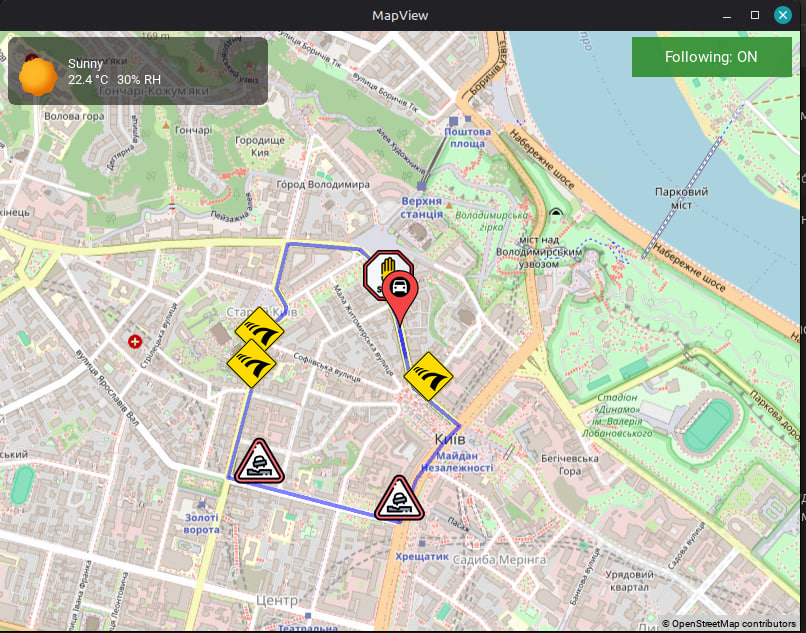
\includegraphics[width=0.82\textwidth]{images/4.jpg}
\caption{Główny ekran aplikacji MapView: pozycja pojazdu, przebyta trasa oraz
  markery wykrytych defektów (dziury, wyboje, gwałtowne hamowanie).}
\label{fig:ss-overview}
\end{figure}

\begin{figure}[H]
\centering
\begin{minipage}[c]{0.6\textwidth}\centering
  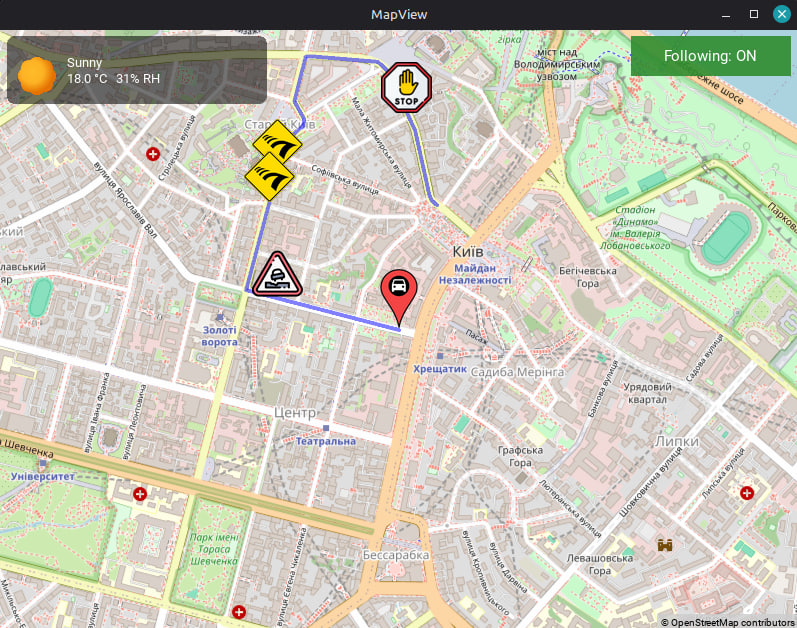
\includegraphics[width=\linewidth]{images/3.jpg}
\end{minipage}\hfill
\begin{minipage}[c]{0.36\textwidth}\centering
  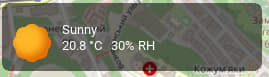
\includegraphics[width=\linewidth]{images/5.jpg}
\end{minipage}
\caption{Markery defektów na trasie — znak STOP (gwałtowne hamowanie), wyboje i
  dziury (po lewej) oraz widget warunków pogodowych z piktogramem i odczytami
  temperatury i wilgotności (po prawej).}
\label{fig:ss-details}
\end{figure}

\begin{figure}[H]
\centering
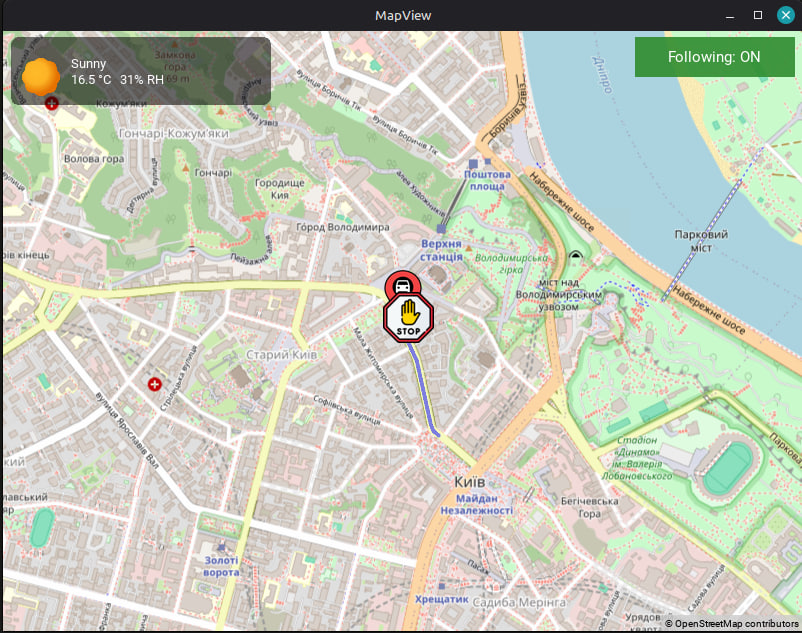
\includegraphics[width=0.78\textwidth]{images/1.jpg}
\caption{Tryb śledzenia pojazdu (Following: ON) — mapa automatycznie centruje się
  na bieżącej pozycji pojazdu.}
\label{fig:ss-follow}
\end{figure}

\subsection{Wybrane decyzje projektowe UX}
\begin{itemize}[leftmargin=1.4em, itemsep=2pt]
  \item Siatka przestrzenna (komórki ok.~30$\times$30~m) zapobiega
        wielokrotnemu oznaczaniu tego samego ubytku przy ponownym przejeździe.
  \item Tryb śledzenia pojazdu można włączać/wyłączać jednym przyciskiem.
  \item Automatyczny reset trasy przy „przeskoku” GPS powyżej 500~m
        zapobiega rysowaniu nieprawdziwych, długich odcinków.
\end{itemize}

%==============================================================================
\section{Testowanie i weryfikacja}
%==============================================================================
Weryfikację prowadzono na danych odtwarzanych z plików CSV, co zapewniło
powtarzalność scenariuszy. Testy obejmowały zarówno poprawność klasyfikacji, jak i
działanie całego potoku „od końca do końca”.

\begin{table}[H]
\centering
\caption{Wybrane scenariusze testowe}
\renewcommand{\arraystretch}{1.2}
\begin{tabularx}{\textwidth}{c X p{3.6cm} c}
\toprule
\rowcolor{rvHead}\textbf{\#} & \textbf{Scenariusz} & \textbf{Oczekiwany wynik} & \textbf{Status} \\
\midrule
T1 & Odczyt akcelerometru w normie & Stan „równa” & \textcolor{rvGreen}{OK} \\
T2 & Duże ujemne odchylenie osi Z & Stan „wyboj” & \textcolor{rvGreen}{OK} \\
T3 & Dodatnie odchylenie osi Z & Stan „dziura” & \textcolor{rvGreen}{OK} \\
T4 & Odczyt z $=0$ & „gwałtowne hamowanie” & \textcolor{rvGreen}{OK} \\
T5 & Pełny potok Agent$\rightarrow$MapView & Marker na mapie & \textcolor{rvGreen}{OK} \\
T6 & Ponowny przejazd tą samą ulicą & Brak duplikatu markera & \textcolor{rvGreen}{OK} \\
\bottomrule
\end{tabularx}
\end{table}

%==============================================================================
\section{Podsumowanie i wnioski}
%==============================================================================

\subsection{Realizacja celów}
Wszystkie założone wymagania funkcjonalne zostały zrealizowane: powstał kompletny,
działający potok przetwarzania danych — od akwizycji w pojeździe, przez
klasyfikację brzegową i trwały zapis, po wizualizację w czasie rzeczywistym na
mapie miasta. Projekt ukończono w zaplanowanym oknie czasowym (05.05--09.06.2026).

\subsection{Wnioski z pracy zespołowej}
Najważniejszym wnioskiem jest skuteczność wczesnej integracji oraz
redundancji kompetencji jako technik zabezpieczających. Dzięki
zbudowaniu szkieletu „end-to-end” na wczesnym etapie zespół wykrył problemy
interfejsów (najwyżej ocenione ryzyko R2) zanim stały się kosztowne. Konteneryzacja
wyeliminowała klasę błędów „u mnie działa”. Elastyczny podział obowiązków pomiędzy
przedmiotami pozwolił efektywnie wykorzystać mocne strony obu członków zespołu.
Zastosowane techniki — WBS, wykres Gantta, analiza ścieżki krytycznej, rejestr
ryzyka i macierz RACI — okazały się adekwatne nawet dla małego zespołu i znacząco
zwiększyły przewidywalność prac.

\subsection{Kierunki rozwoju}
\begin{itemize}[leftmargin=1.4em, itemsep=2pt]
  \item Zastąpienie odtwarzania z CSV strumieniem z rzeczywistego urządzenia IoT.
  \item Uczenie maszynowe do klasyfikacji nawierzchni zamiast progów stałych.
  \item Agregacja danych od wielu pojazdów (mapa zbiorcza dla miasta).
  \item Wersja webowa lub mobilna aplikacji MapView.
\end{itemize}

%==============================================================================
\addcontentsline{toc}{section}{Bibliografia}
\begin{thebibliography}{9}
\bibitem{pmbok} Project Management Institute, \emph{A Guide to the Project
  Management Body of Knowledge (PMBOK Guide)}, wyd.~6, PMI, 2017.
\bibitem{kerzner} H.~Kerzner, \emph{Project Management: A Systems Approach to
  Planning, Scheduling, and Controlling}, Wiley, 2017.
\bibitem{fastapi} S.~Ramírez, \emph{FastAPI — dokumentacja oficjalna}.
  \url{https://fastapi.tiangolo.com}
\bibitem{mqtt} OASIS, \emph{MQTT Version 3.1.1 — specyfikacja protokołu}, 2014.
\bibitem{redis} \emph{Redis — dokumentacja}. \url{https://redis.io/docs}
\bibitem{postgres} \emph{PostgreSQL 16 — dokumentacja}.
  \url{https://www.postgresql.org/docs/16/}
\bibitem{kivy} \emph{Kivy — Cross-platform Python Framework}.
  \url{https://kivy.org}
\bibitem{docker} \emph{Docker Compose — dokumentacja}.
  \url{https://docs.docker.com/compose/}
\bibitem{cockburn} A.~Cockburn, \emph{Hexagonal Architecture (Ports and
  Adapters)}, 2005.
\end{thebibliography}

\newpage
\addcontentsline{toc}{section}{Spis rysunków}
\listoffigures
\addcontentsline{toc}{section}{Spis tablic}
\listoftables

\end{document}
